%%%%%%%%%%%%%%%%%%%%%%%%%%%%%%%%%%%%%%%%%%%%%%%%%%%%%%%%%%%%%%%%%%%%%%%%%%%

\chapter{Vectors and Matrices}


%%%%%%%%%%%%%%%%%%%%%%%%%%%%%%%%%%%%%%%%%%%%%%%%%%%%%%%%%%%%%%%%%%%%%%%%%%%

\section{Scalars and vectors}
\label{sec:scalars_vectors}

The path of a car travelling from location $A$ to location $B$ is
characterized by two quantities or \emph{scalars}\index{scalars}: a
magnitude\index{magnitude}~(such as speed), and a direction~(from $A$
to $B$). Both of these two scalars are summarized by a
\emph{vector}\index{vector}.

\begin{figure}[!htpb]
\centering
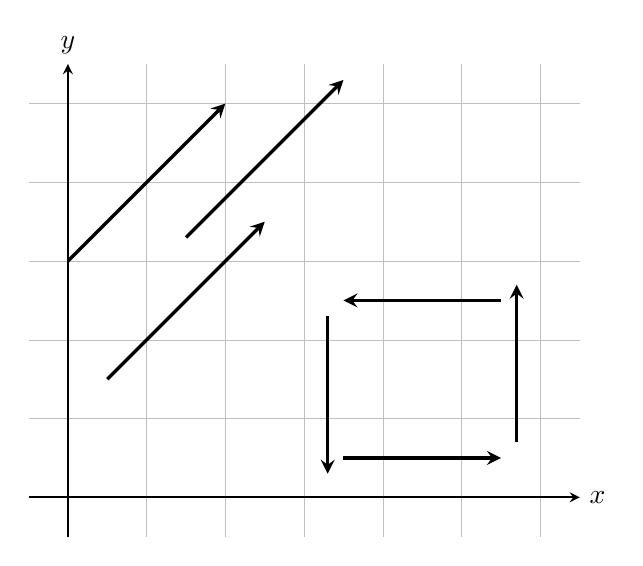
\begin{tikzpicture}
[linedecorate/.style={->,>=stealth,very thick}]
% grids for the plane
\draw[step=1cm,lightgray,very thin] (-0.5,-0.5) grid (6.5,5.5);
% the rectangular axes
\draw[->,>=stealth,semithick] (-0.5,0) -- (6.5,0) node[right]{$x$};
\draw[->,>=stealth,semithick] (0,-0.5) -- (0,5.5) node[above]{$y$};
% vectors
\draw[linedecorate] (0,3) -- node[above left]{$\vecu$} (2,5);
\draw[linedecorate] (1.5,3.3) -- node[below right]{$\vecv$} (3.5,5.3);
\draw[linedecorate] (0.5,1.5) -- node[below right]{$\vecw$} (2.5,3.5);
\draw[linedecorate] (3.5,0.5) -- (5.5,0.5);
\draw[linedecorate] (5.7,0.7) -- (5.7,2.7);
\draw[linedecorate] (5.5,2.5) -- (3.5,2.5);
\draw[linedecorate] (3.3,2.3) -- (3.3,0.3);
\end{tikzpicture}
\caption{Vectors in the $x$-$y$ plane.}
\label{fig:vectors_matrices:plane_vectors}
\end{figure}

In the $x$-$y$ plane, we can visualize a vector as an arrow from point
$A$ to point $B$~(see
Figure~\ref{fig:vectors_matrices:plane_vectors}). The starting point
$A$ of the vector is called the \emph{tail}\index{vectors!tail} and
the terminal point $B$ is the \emph{head}.\index{vectors!head} Two
vectors are \emph{equivalent}\index{vectors!equivalent} if they have
the same magnitude and direction. The vectors $\vecu$, $\vecv$, and
$\vecw$ in Figure~\ref{fig:vectors_matrices:plane_vectors} are thus
all equivalent to each other.

To analyze vectors using algebra, we can think of a vector $\vecu$
as starting from the origin of the $x$-$y$ plane and having
$(u_1, u_2)$ as the coordinate for its head~(see
Figure~\ref{fig:specify_vector_head_coordinate}). So $\vecu$ is
completely determined by the coordinate of its head and we write
$\vecu = \langle u_1, u_2 \rangle$ as an algebraic representation
for $\vecu$.

\begin{figure}[!htpb]
\centering
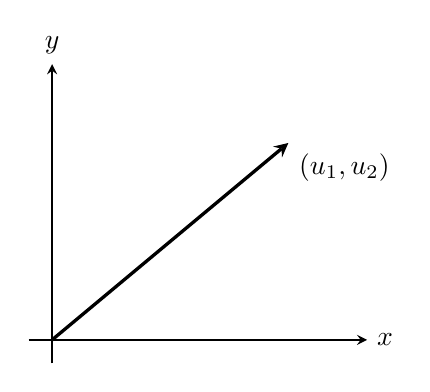
\begin{tikzpicture}
% the rectangular axes
\draw[->,>=stealth,semithick] (-0.3,0) -- (4,0) node[right]{$x$};
\draw[->,>=stealth,semithick] (0,-0.3) -- (0,3.5) node[above]{$y$};
% vector described by its head coordinate
\draw[->,>=stealth,very thick] (0,0) -- node[above left]{$\vecu$} (3,2.5) node[below right]{$(u_1, u_2)$};
\end{tikzpicture}
\caption{A vector as specified by its head coordinate.}
\label{fig:specify_vector_head_coordinate}
\end{figure}

In case the tail of $\vecu$ is not the origin, we let $(x_1, y_1)$
be the coordinate of the tail and denote the coordinate of the head by
$(x_2, y_2)$. By subtracting coordinatewise, we obtain an equivalent
vector $\vecv$ that emanates from the origin of the $x$-$y$
plane. The coordinate of $\vecv$ is
\[
(x_2, y_2) - (x_1, y_1)
=
(x_2 - x_1,\; y_2 - y_1)
=
(u_1, u_2)
\]
and we do not distinguish between $\vecu$ and $\vecv$. Thus we
can transform $\vecu$ to be a vector emanating from the origin and
specified by the coordinate
%
\begin{equation}
\label{eq:component_form_vector}
\vecu
=
\langle x_2 - x_1,\; y_2 - y_1 \rangle
=
\langle u_1, u_2 \rangle.
\end{equation}
%
Equation~(\ref{eq:component_form_vector}) is called the
\emph{component form}\index{component form} of a vector, with $u_1$
and $u_2$ being the individual components. The vector
$\veczero = \langle 0, 0 \rangle$ is called the zero
vector.\index{zero vector}

\begin{figure}[!htpb]
\centering
\begin{tikzpicture}
% the rectangular axes
\draw[->,>=stealth,semithick] (-2.5,0) -- (5.7,0) node[right]{$x$};
\draw[->,>=stealth,semithick] (0,-1.5) -- (0,6.7) node[above]{$y$};
% ticks on horizontal axis
\foreach \x in {-2,-1,-1}
  \draw (\x cm,2pt) -- (\x cm,-2pt) node[anchor=north] {$\x$};
\foreach \x in {1,2,...,5}
  \draw (\x cm,2pt) -- (\x cm,-2pt) node[anchor=north] {$\x$};
% ticks on vertical axis
\foreach \y in {-1,-1}
  \draw (2pt,\y cm) -- (-2pt,\y cm) node[anchor=east] {$\y$};
\foreach \y in {1,2,...,6}
  \draw (2pt,\y cm) -- (-2pt,\y cm) node[anchor=east] {$\y$};
% vector u
\draw[->,>=stealth,very thick] (-2,-1) node[below]{$(-2,-1)$} -- node[above left]{$\vecu$} (1,3) node[above]{$(1,3)$};
% vector v
\draw[->,>=stealth,very thick] (1.5,1.5) node[below]{$(1.5,1.5)$} -- node[above left]{$\vecv$} (4.5,5.5) node[above]{$(4.5,5.5)$};
\end{tikzpicture}
\caption{Verify that vectors $\vecu$ and $\vecv$ are equivalent.}
\label{fig:vectors_matrices:verify_vectors_u_v}
\end{figure}

\begin{example}
Let the vector $\vecu$ be described by the directed line segment
from $(-2,-1)$ to $(1,3)$, and let $\vecv$ be the line segment from
$(1.5,1.5)$ to $(4.5,5.5)$, as shown in
Figure~\ref{fig:vectors_matrices:verify_vectors_u_v}. Show that
$\vecu$ and $\vecv$ are equivalent vectors.
\end{example}

\begin{proof}[Solution]
To show that $\vecu$ and $\vecv$ are equivalent, we need to show
that they have the same length and are in the same direction. The
length of $\vecu$ is equivalent to the length of the line segment
from $(-2,-1)$ to $(1,3)$:
%
\begin{align*}
\sqrt{(1 - (-2))^2 + (3 - (-1))^2}
&=
\sqrt{(1 + 2)^2 + (3 + 1)^2} \\
&=
\sqrt{9 + 16} \\
&=
5.
\end{align*}
%
This tells us that $\vecu$ has length 5. Similarly, the length of
$\vecv$ is
%
\begin{align*}
\sqrt{(4.5 - 1.5)^2 + (5.5 - 1.5)^2}
&=
\sqrt{3^2 + 4^2} \\
&=
\sqrt{9 + 16} \\
&=
5
\end{align*}
%
which is the same length as that of $\vecu$.

\begin{lstlisting}
sage: u = vector([1 - (-2), 3 - (-1)]); u
(3, 4)
sage: v = vector([4.5 - 1.5, 5.5 - 1.5]); v
(3.000...000, 4.000...000)
sage: u.norm()
5
sage: v.norm()
5.000...000
\end{lstlisting}

The slope of the line segment from $(-2,-1)$ to $(1,3)$ is
\[
\frac{3 - (-1)} {1 - (-2)}
=
\frac{4}{3}
\]
and the slope of the line segment from $(1.5,1.5)$ to $(4.5,5.5)$ is
\[
\frac{5.5 - 1.5}{4.5 - 1.5}
=
\frac{4}{3}
\]
which shows that these two line segments have the same direction, so
$\vecu$ and $\vecv$ point in the same direction.
%
\begin{lstlisting}
sage: (3 - (-1)) / (1 - (-2))
4/3
sage: (5.5 - 1.5) / (4.5 - 1.5)
1.333...333
sage: QQ((5.5 - 1.5) / (4.5 - 1.5))
4/3
\end{lstlisting}
%
Therefore, $\vecu$ and $\vecv$ are equivalent vectors.
\end{proof}

We denote the length of a vector as follows. Let $\vecu$ be a
vector whose starting point is $P = (x_1, y_1)$ and whose terminal
point is $Q = (x_2, y_2)$. Then the length or magnitude of $\vecu$
is denoted by $\vecvertl \vecu \vecvertr$ and given
by the equation
%
\begin{equation}
\label{eq:vectors_matrices:magnitude_two_dimensional_vector}
\begin{aligned}
\vecvertl \vecu \vecvertr
&=
\sqrt{(x_2 - x_1)^2 + (y_2 - y_1)^2} \\
&=
\sqrt{v_1^2 + v_2^2}.
\end{aligned}
\end{equation}


%%%%%%%%%%%%%%%%%%%%%%%%%%%%%%%%%%%%%%%%%%%%%%%%%%%%%%%%%%%%%%%%%%%%%%%%%%%

\section{Add, subtract, and multiply vectors}
\index{vectors!arithmetic}
%% Relate vectors with complex numbers.

The left-hand side of Figure~\ref{fig:vectors_matrices:vector_sum}
illustrates the path of an object. Initially travelling in the
direction of vector $\vecu$, the object then changes its direction to
move in the direction of $\vecv$. The total displacement of the object
is represented as the vector $\vecu + \vecv = \vecw$. Furthermore, we
could first go in the direction of $\vecv$ and then in that of $\vecu$,
and hence obtain the same displacement $\vecv + \vecu = \vecw$, as
shown on the right-hand side of
Figure~\ref{fig:vectors_matrices:vector_sum}. This ``adding'' of
vectors is just one of many basic operations that can be performed on
vectors. In fact, the ``adding'' rule illustrated in
Figure~\ref{fig:vectors_matrices:vector_sum} is called the
\emph{parallelogram rule}\index{parallelogram rule} for vector
addition.

\begin{figure}[!htpb]
\centering
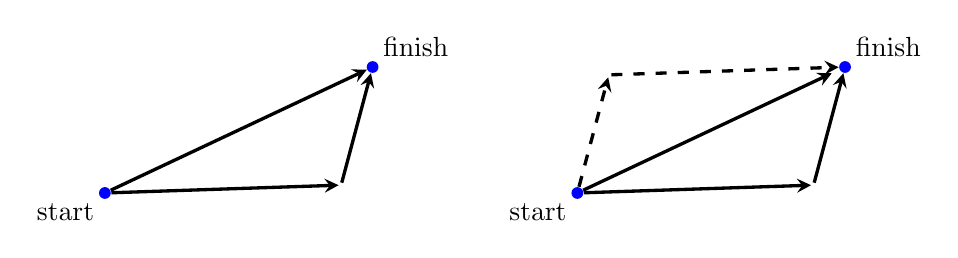
\begin{tikzpicture}
% left set of vectors
\node (start1) at (0,0) [circle,fill=blue,inner sep=1.5pt]{};
\node (middle1) at (3,0.1) [circle,inner sep=0.5pt]{};
\node (finish1) at (3.4,1.6) [circle,fill=blue,inner sep=1.5pt]{};
\draw[->,>=stealth,very thick] (start1) node[below left]{start}  -- node[below]{$\vecu$} (middle1);
\draw[->,>=stealth,very thick] (middle1) -- node[right]{$\vecv$} (finish1) node[above right]{finish};
\draw[->,>=stealth,very thick] (start1) -- node[above]{$\vecw$} (finish1);
% right set of vectors
\node (start2) at (6,0) [circle,fill=blue,inner sep=1.5pt]{};
\node (lowerMiddle) at (9,0.1) [circle,inner sep=0.5pt]{};
\node (upperMiddle) at (6.4,1.5) [circle,inner sep=0.5pt]{};
\node (finish2) at (9.4,1.6) [circle,fill=blue,inner sep=1.5pt]{};
\draw[->,>=stealth,very thick] (start2) node[below left]{start} -- node[below]{$\vecu$} (lowerMiddle);
\draw[->,>=stealth,very thick] (lowerMiddle) -- node[right]{$\vecv$} (finish2) node[above right]{finish};
\draw[->,>=stealth,shorten >=3pt,very thick] (start2) -- node[above]{$\vecw$} (finish2);
\draw[->,>=stealth,very thick,dash pattern=on 4pt off 4pt] (start2) -- node[left]{$\vecv$} (upperMiddle);
\draw[->,>=stealth,very thick,dash pattern=on 4pt off 4pt] (upperMiddle) -- node[above]{$\vecu$} (finish2);
\end{tikzpicture}
\caption{The vector sum $\vecu + \vecv = \vecw = \vecv + \vecu$.}
\label{fig:vectors_matrices:vector_sum}
\end{figure}

\begin{definition}
\label{def:vectors_matrices:vector_operations}
Let $\vecu = \langle u_1, u_2 \rangle$ and
$\vecv = \langle v_1, v_2 \rangle$ be vectors and suppose
$c$ is a scalar. Then we have the following operations on vectors:
\begin{enumerate}
\item The \emph{vector sum} of $\vecu$ and
  $\vecv$ is $\vecu + \vecv = \langle u_1 + v_1,\; u_2 + v_2 \rangle$.

\item The \emph{negative} of $\vecu$ is
  $-\vecu = \langle -u_1, -u_2 \rangle$.

\item The \emph{vector difference} of $\vecu$ and
  $\vecv$ is $\vecu - \vecv =
  \langle u_1, u_2 \rangle - \langle v_1, v_2 \rangle = \langle u_1 -
  v_1,\; u_2 - v_2 \rangle$.

\item The \emph{scalar multiple} of $c$ and $\vecu$ is
  $c\vecu = \langle c u_1, c u_2 \rangle$.
\end{enumerate}
\end{definition}

The negative of a vector $\vecu$ is a vector that has the same
length as $\vecu$, but goes in the opposite direction. One
exception is the zero vector $\veczero$, whose negative is itself
because $-\veczero = -\langle 0,0 \rangle = \langle -0, -0 \rangle =
\langle 0,0 \rangle = \veczero$. More generally, scalar
multiplication has the effect of scaling a vector. This may result in
expanding the vector, contracting it, producing the negative of the
vector, or expanding/contracting the negative of the vector. These
various possibilities are shown in
Figure~\ref{fig:scalar_multiply_negative}.

\begin{figure}[!htpb]
\centering
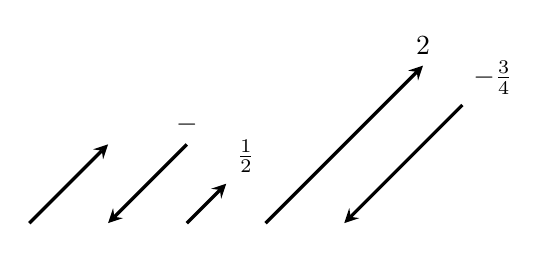
\begin{tikzpicture}
\draw[->,>=stealth,very thick] (0,0) -- (1,1) node[above]{$\vecu$};
\draw[<-,>=stealth,very thick] (1,0) -- (2,1) node[above]{$-\vecu$};
\draw[->,>=stealth,very thick] (2,0) -- (2.5,0.5) node[above right]{$\frac{1}{2}\vecu$};
\draw[->,>=stealth,very thick] (3,0) -- (5,2) node[above]{$2\vecu$};
\draw[<-,>=stealth,very thick] (4,0) -- (5.5,1.5) node[above right]{$-\frac{3}{4}\vecu$};
\end{tikzpicture}
\caption{Scalar multiplication and negative of a vector.}
\label{fig:scalar_multiply_negative}
\end{figure}

Using the parallelogram rule for vector addition, we can similarly
illustrate vector difference. The left-hand side of
Figure~\ref{fig:vectors_matrices:vector_difference_parallelogram_triangle} shows the
parallelogram rule for vector subtraction, while the right-hand side shows
the triangle rule for vector subtraction. Thus to determine the
difference of two vectors $\vecu$ and $\vecv$, we first align the
vectors so that their initial points coincide. Then the difference
$\vecu - \vecv$ is the vector that starts from the head of
$\vecv$ and ends at the terminal point of $\vecu$.

\begin{figure}[!htpb]
\centering
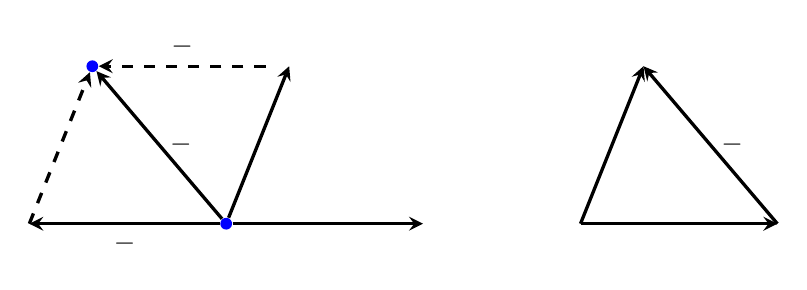
\begin{tikzpicture}
% left-hand figure: vector difference by parallelogram rule
\node (origin) at (0,0) [circle,fill=blue,inner sep=1.5pt]{};
\node (destin) at (-1.7,2) [circle,fill=blue,inner sep=1.5pt]{};
\draw[->,>=stealth,very thick] (origin) -- node[below]{$\vecv$} (2.5,0);
\draw[->,>=stealth,very thick] (origin) -- node[below]{$-\vecv$} (-2.5,0);
\draw[->,>=stealth,very thick] (origin) -- node[right]{$\vecu$} (0.8,2);
\draw[->,>=stealth,very thick,dash pattern=on 4pt off 4pt] (-2.5,0) -- node[left]{$\vecu$} (destin);
\draw[->,>=stealth,very thick,dash pattern=on 4pt off 4pt] (0.5,2) -- node[above]{$-\vecv$} (destin);
\draw[->,>=stealth,very thick] (origin) -- node[right]{$\vecu - \vecv$} (destin);
% right-hand figure: vector difference
\draw[->,>=stealth,very thick] (4.5,0) -- node[left]{$\vecu$} (5.3,2);
\draw[->,>=stealth,very thick] (4.5,0) -- node[below]{$\vecv$} (7,0);
\draw[->,>=stealth,very thick] (7,0) -- node[right]{$\vecu - \vecv$} (5.3,2);
\end{tikzpicture}
\caption{Vector difference by the parallelogram rule~(left) and by the
triangle rule~(right).}
\label{fig:vectors_matrices:vector_difference_parallelogram_triangle}
\end{figure}

Vector operations share many of the familiar properties of operations
on real numbers. Given two real numbers, for example, it does not
matter in which order we add
them. Problem~\ref{prob:vectors_matrices:field_laws_for_vectors} lists
a number of vector rules that are similar to those obeyed by real numbers.

\begin{example}
Using vector rules from
problem~\ref{prob:vectors_matrices:field_laws_for_vectors}, find a
vector $\vecx$ such that $5\vecx + 7\vecu = 4\vecv$.
\end{example}

\begin{proof}[Solution]
First, subtract $7\vecu$ from both sides of the equal sign to get
$5\vecx + (7\vecu - 7\vecu) = 4\vecv - 7\vecu$, which can be
simplified to $5\vecx = 4\vecv - 7\vecu$. Now divide both sides of
the last equation by $5$ and we have
$\frac{1}{5} (5\vecx) = \frac{1}{5} (4\vecv - 7\vecu)$. Simplify the
last equation to
$\vecx = \frac{1}{5} (4\vecv) + \frac{1}{5}(-7\vecu)$. So the required
vector is $\vecx = \frac{4}{5}\vecv - \frac{7}{5}\vecu$.
\end{proof}

Any nonzero vector $\vecv$ can be transformed into a vector $\vecu$ of
magnitude $1$. The equation to effect this transformation is
%
\begin{equation}
\label{eq:vectors_matrices:two_dimensional_unit_vector}
\vecu
=
\frac {\vecv} {\vecvertl \vecv \vecvertr}
=
\vecv
\frac {1} {\vecvertl \vecv \vecvertr}.
\end{equation}
%
The process of using
equation~(\ref{eq:vectors_matrices:two_dimensional_unit_vector}) to
transform a nonzero vector into a vector of magnitude $1$ is called
\emph{normalizing}\index{vectors!normalization} a vector. For example,
given the vector $\vecu = \langle 1, 2 \rangle$, we can use
equation~(\ref{eq:vectors_matrices:two_dimensional_unit_vector}) to
find the normalized form of $\vecu$. Since
$\vecvertl \vecu \vecvertr = \sqrt{5}$ by
equation~(\ref{eq:vectors_matrices:magnitude_two_dimensional_vector}),
so $\vecu$ is normalized as
%
\begin{align*}
\frac {\vecu} {\vecvertl \vecu \vecvertr}
&=
\frac{1}{\sqrt{5}} \langle 1, 2 \rangle \\[4pt]
&=
\frac{\sqrt{5}}{5} \langle 1, 2 \rangle.
\end{align*}

\begin{lstlisting}
sage: u = vector([1, 2])
sage: u / u.norm()
(1/5*sqrt(5), 2/5*sqrt(5))
\end{lstlisting}


%%%%%%%%%%%%%%%%%%%%%%%%%%%%%%%%%%%%%%%%%%%%%%%%%%%%%%%%%%%%%%%%%%%%%%%%%%%

\subsection{Applications to geometry}
\label{subsec:2D_vectors_apply_geometry}

A line in the $x$-$y$ plane is usually described by the linear
equation
\[
y = mx + c
\]
where $m \neq 0$ is the slope of the line and $c$ is a constant. The
same line can be represented in \emph{vector form}\index{vector form}
as
%
\begin{equation}
\label{eq:vector_form_line}
\langle x,\, mx + c \rangle
=
\langle 0, c \rangle + x \langle 1, m \rangle.
\end{equation}
%
The vector $\langle 0, c \rangle$ points to the line, while the vector
$\langle 1, m \rangle$ is in the same direction as the line.

\begin{example}
Express the line $2x + 3y = 4$ in vector form.
\end{example}

\begin{proof}[Solution]
Solving the equation $2x + 3y = 4$ for $y$ to get
\[
y = \frac{4}{3} - \frac{2}{3} x.
\]
Using equation~(\ref{eq:vector_form_line}), we have
\[
\langle 0,\, 4/3 \rangle
+ x \langle 1,\, -2/3 \rangle
\]
which is a representation of the line $2x + 3y = 4$ in vector form.
\end{proof}

In general, a line $L$ has many different vector representations. If
$(u_1, u_2)$ is a point on $L$, then $\vecu = \langle u_1, u_2
\rangle$ is a vector pointing to $L$. Furthermore, let $\vecv =
\langle v_1, v_2 \rangle$ be a vector in the same direction as
$L$. Then the line $L$ can be represented in vector form as
\[
\langle x, y \rangle
=
\vecu + t \vecv
\]
with $t$ being a parameter.

Two nonzero vectors $\vecu$ and $\vecv$ are said to be
\emph{linearly dependent}\index{linearly dependent} if they can be
expressed as a linear combination that equals the zero vector, i.e. we
can find two nonzero real numbers $m,n$ such that
$m\vecu + n\vecv = \veczero$. From this definition, it follows that
two vectors are parallel if and only if they are linearly
dependent. In other words, if two vectors are parallel then they are
linearly dependent. The converse is also true: if two vectors are
linearly dependent, then they are parallel.


%%%%%%%%%%%%%%%%%%%%%%%%%%%%%%%%%%%%%%%%%%%%%%%%%%%%%%%%%%%%%%%%%%%%%%%%%%%

\section{Three-dimensional vectors}
\index{vectors!three-dimensional}

Just as vectors in the plane are described by two components, so
vectors in three-dimensional space are described by three components,
as shown in Figure~\ref{fig:vectors_matrices:3D_vector}. If $\vecu$ is
a vector whose tail is the origin $(0,0,0)$ and whose head is
$(u_1, u_2, u_3)$, then the \emph{component form} of $\vecu$ is
$\vecu = \langle u_1, u_2, u_3 \rangle$. Moving from two dimensions to
three does not change many of the vector results presented earlier in
this chapter. In fact, the magnitude of $\vecu$ is similarly defined as
%
\begin{equation}
\label{eq:vectors_matrices:magnitude_three_dimensional_vector}
\vecvertl \vecu \vecvertr
=
\sqrt{u_1^2 + u_2^2 + u_3^2}
\end{equation}
%
and if $\vecu \neq \veczero$ then its \emph{normalized form} is
%
\begin{equation}
\label{eq:normalize_vector_three_dimensions}
\frac{\vecu}{\vecvertl \vecu \vecvertr}
=
\vecu \frac{1}{\vecvertl \vecu \vecvertr}.
\end{equation}
%
Definition~\ref{def:vectors_matrices:vector_operations} can be easily
cast in terms of vectors in three-dimensional space; we simply add an
extra component.

\begin{figure}[!htpb]
\centering
%% \begin{pspicture}(-1,-2)(4,4)
%% \pstThreeDCoor[linecolor=black,Alpha=-280,xMin=-0.5,xMax=4,yMin=-0.5,yMax=4,zMin=-0.5,zMax=4]
%% \pstThreeDDot[linecolor=blue,dotsize=4pt](1,4,5)\uput[0](2,2.8){$(u_1, u_2, u_3)$}
%% \pstThreeDLine[linewidth=1.5pt,arrows=->](0,0,0)(1,4,5)\uput[0](0.5,1.5){$\vecu$}
%% \pstThreeDLine[linewidth=0.5pt,linecolor=blue,linestyle=dashed](0,0,0)(1,4,0)
%% \pstThreeDLine[linewidth=0.5pt,linecolor=blue,linestyle=dashed](1,4,0)(1,4,5)
%% \end{pspicture}
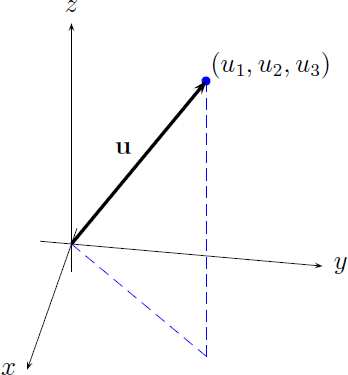
\includegraphics[scale=0.8]{images/vector-3d}
\caption{A vector in three-dimensional space.}
\label{fig:vectors_matrices:3D_vector}
\end{figure}

%% \begin{practice}
%% Let \emph{\vecu} be a three-dimensional vector and let $c$ be a
%% scalar. Show that $\vecvertl c \emph{\vecu}
%% \vecvertr = |c| \, \vecvertl \emph{\vecu}
%% \vecvertr$.
%% \end{practice}

%% \begin{practice}
%% \label{prac:triangle_inequality_three_dimensions}
%% Given two vectors $\emph{\vecu} = \langle 3, 5, 7 \rangle$ and
%% $\emph{\textbf{v}} = \langle -1, 2, 9 \rangle$, show that
%% $\vecvertl \emph{\vecu} + \emph{\textbf{v}}
%% \vecvertr \leq \vecvertl \emph{\vecu}
%% \vecvertr + \vecvertl \emph{\textbf{v}} \vecvertr$.
%% \end{practice}

\begin{figure}[!htpb]
\centering
%% \begin{pspicture}(-3,-1)(3,3)
%% \pstThreeDCoor[linecolor=black,xMin=-0.5,xMax=3,yMin=-0.5,yMax=3,zMin=-0.5,zMax=3]
%% \pstThreeDLine[linewidth=1.5pt,arrows=->](0,0,0)(2,0,0)
%% \pstThreeDLine[linewidth=1.5pt,arrows=->](0,0,0)(0,2,0)
%% \pstThreeDLine[linewidth=1.5pt,arrows=->](0,0,0)(0,0,2)
%% \uput[0](-2.7,-0.5){$(1,0,0)$}\uput[0](-1,-0.1){\veci}
%% \uput[0](1.2,-0.4){$(0,1,0)$}\uput[0](0.5,0){\vecj}
%% \uput[0](-0.1,1.8){$(0,0,1)$}\uput[0](0,1){\veck}
%% \end{pspicture}
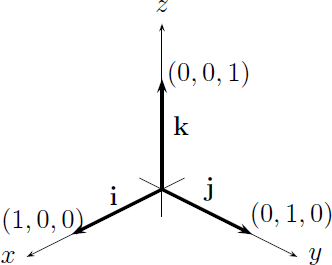
\includegraphics[scale=0.8]{images/unit-vectors-3d}
\caption{Unit vectors in three-dimensional space.}
\label{fig:vectors_matrices:unit_vectors_3D}
\end{figure}

If a nonzero vector $\vecu$ (in two- or three-dimensional space) is
multiplied by $1 / \vecvertl \vecu \vecvertr$, the result is a vector
of magnitude $1$. Vectors of magnitude $1$ are called
\emph{unit vectors}\index{unit vectors}. Thus the vector in
equation~(\ref{eq:vectors_matrices:two_dimensional_unit_vector}) is a
two-dimensional unit vector. Of particular interest in physics are the
\emph{standard unit vectors}\index{standard unit vectors}
\[
\veci = \langle 1, 0 \rangle
\qquad\text{and}\qquad
\vecj = \langle 0, 1 \rangle
\]
in the two-dimensional plane, and their three-dimensional
counterparts:
%
\begin{equation}
\label{eq:vectors_matrices:standard_unit_vectors_three_dimensions}
\veci = \langle 1, 0, 0 \rangle, \qquad
\vecj = \langle 0, 1, 0 \rangle, \qquad
\veck = \langle 0, 0, 1 \rangle.
\end{equation}
%
The three-dimensional standard unit vectors are shown in
Figure~\ref{fig:vectors_matrices:unit_vectors_3D}. These vectors play
a role similar to the number $1$, where every real number $a$ can be
expressed as $a = a \cdot 1$. So every three-dimensional~(respectively
two-dimensional) vector $\vecu = \langle u_1, u_2, u_3 \rangle$ can be
expressed in terms of the standard unit
vectors~(\ref{eq:vectors_matrices:standard_unit_vectors_three_dimensions})
as
\[
\vecu
=
\langle u_1, u_2, u_3 \rangle
=
\langle u_1, 0, 0 \rangle +
\langle 0, u_2, 0 \rangle + \langle 0, 0, u_3 \rangle
=
u_1 \veci + u_2 \vecj + u_3 \veck.
\]
For example, in the plane we have
$\langle 2, 3 \rangle = 2\veci + 3 \vecj$. In three-dimensional space
we have $\langle 5, -1, 7 \rangle = 5 \veci - \vecj + 7 \veck$, whose
magnitude is $5\sqrt{3}$ and so
\[
\frac{1}{5\sqrt{3}} \langle 5, -1, 7 \rangle
=
\frac{1}{\sqrt{3}}\veci
-
\frac{1}{5\sqrt{3}}\vecj
+
\frac{7}{5\sqrt{3}}\veck
\]
is a unit vector in the same direction as $\langle 5, -1, 7 \rangle$.


%%%%%%%%%%%%%%%%%%%%%%%%%%%%%%%%%%%%%%%%%%%%%%%%%%%%%%%%%%%%%%%%%%%%%%%%%%%

\section{The dot product}
\label{sec:dot_product}
\index{dot product}

Section~\ref{sec:scalars_vectors} discussed vectors and
showed how we can perform various arithmetic operations on them. In
particular, we have shown how a vector can be multiplied by a
scalar. We now consider the case of multiplying two vectors.

\begin{definition}
\label{def:vectors_matrices:vector_dot_product}
Let $\vecu = \langle u_1, u_2, u_3 \rangle$ and
$\vecv = \langle v_1, v_2, v_3 \rangle$ be
three-dimensional vectors. Then the vector \emph{dot product}
of $\vecu$ and $\vecv$ is defined as
\[
\vecu \cdot \vecv
=
u_1 v_1 + u_2 v_2 + u_3 v_3.
\]
\end{definition}

The vector dot product is also called the scalar or inner
product\index{scalar product}\index{inner product}. Unlike scalar
multiplication of a scalar $c$ and a vector $\vecu$, which results
in another vector $c\vecu$, the dot product of two vectors
$\vecu$ and $\vecv$ is a scalar. A similar definition holds for
two-dimensional vectors. Thus to find the dot product of two vectors
both of which are in two- or three-dimensional space, we multiply the
corresponding components and add up the results.

\begin{lstlisting}
sage: u = vector([3, 5, 7])
sage: v = vector([-2, 7, -9])
sage: # compute dot product from definition
sage: zip(u, v)
[(3, -2), (5, 7), (7, -9)]
sage: p = map(prod, zip(u, v)); p
[-6, 35, -63]
sage: sum(p)
-34
sage: # compute dot product using built-in functions
sage: u.dot_product(v)
-34
sage: u * v
-34
\end{lstlisting}

We can also find the dot product of two vectors in terms of the angle
between them. If $\theta$ is the angle between two vectors $\vecu$
and $\vecv$ in two- or three-dimensional space, then their dot
product obeys the following geometric interpretation:
\index{dot product!geometric interpretation}
%
\begin{equation}
\label{eq:vectors_matrices:geometric_interpretation_dot_product}
\vecu \cdot \vecv
=
\begin{cases}
\vecvertl \vecu \vecvertr \,
\vecvertl \vecv \vecvertr \cos\theta
&\text{if $\vecu \neq \veczero$ and $\vecv \neq \veczero$}\\
0 & \text{if $\vecu = \veczero$ or $\vecv = \veczero$}.
\end{cases}
\end{equation}
%
Using the last equation, the angle between two nonzero vectors is
given by
%
\begin{equation}
\label{eq:vectors_matrices:angle_between_vectors}
\theta
=
\cos^{-1}
\left(
\frac {\vecu \cdot \vecv}
{\vecvertl \vecu \vecvertr \, \vecvertl \vecv \vecvertr}
\right).
\end{equation}

\begin{example}
Consider the vectors $\vecu = \langle 3, -1, 7 \rangle$
and $\vecv = \langle -2, 5, 8 \rangle$. Find the angle
between $\vecu$ and $\vecv$.
\end{example}

\begin{proof}[Solution]
To find the angle between two vectors, we use
equation~(\ref{eq:vectors_matrices:angle_between_vectors}). From
Definition~\ref{def:vectors_matrices:vector_dot_product}, the dot
product of $\vecu$ and $\vecv$ is
\[
\vecu \cdot \vecv
=
3(-2) + (-1)5 + 7(8)
=
45.
\]
Using
equation~(\ref{eq:vectors_matrices:magnitude_three_dimensional_vector}),
the magnitude of $\vecu$ is
$\vecvertl \vecu \vecvertr = \sqrt{9 + 1 + 49} = \sqrt{59}$ and that
of $\vecv$ is
$\vecvertl \vecv \vecvertr = \sqrt{4 + 25 + 64} = \sqrt{93}$.
Substitute the value of the dot product and the individual magnitudes
into equation~(\ref{eq:vectors_matrices:angle_between_vectors}) to get
\[
\theta
=
\cos^{-1} \left( \frac{45}{\sqrt{59 \cdot 93}} \right)
\]
which is the angle between $\vecu$ and $\vecv$. This angle can
be computed using Sage as follows:
%
\begin{lstlisting}
sage: u = vector([3, -1, 7]); v = vector([-2, 5, 8])
sage: numer = u * v
sage: denom = u.norm() * v.norm()
sage: arccos(numer / denom)
arccos(45/(sqrt(59)*sqrt(93)))
\end{lstlisting}
%
which is the same as what we have above.
\end{proof}

From plane geometry, we know that two lines are perpendicular if the
angle $\theta$ between them is $90^{\circ}$ or $\theta = \pi / 2$
radians. Now $\cos (\pi / 2) = 0$ and using
equation~(\ref{eq:vectors_matrices:geometric_interpretation_dot_product}), we see that
two non-zero vectors are perpendicular (also called
\emph{orthogonal})\index{vectors!orthogonal} if and only if their dot
product is zero.
